\documentclass[a4paper]{article}

%% Language and font encodings
\usepackage[english]{babel}
\usepackage[utf8x]{inputenc}
\usepackage[T1]{fontenc}

%% Sets page size and margins
\usepackage[a4paper,top=3cm,bottom=2cm,left=3cm,right=3cm,marginparwidth=1.75cm]{geometry}

%% Useful packages
\usepackage{amsmath,amssymb}
\usepackage{graphicx}
\graphicspath{ {/home/noa/Pictures} }
\usepackage[colorinlistoftodos]{todonotes}
\usepackage[colorlinks=true, allcolors=blue]{hyperref}
\usepackage{mathtools}
\usepackage{blkarray}
\DeclarePairedDelimiter\bra{\langle}
{\rvert}
\DeclarePairedDelimiter\ket{\lvert}{\rangle}
\DeclarePairedDelimiterX\braket[2]{\langle}{\rangle}{#1 \delimsize\vert #2}
\DeclareMathOperator{\Tr}{Tr}

\begin{document}

Note: I drop constants multiplying the entire expression until I start handling the time dependence.\newline
Before approximations, I have:\newline
\begin{gather*}
(\frac{2}{N+1})^2(\frac{2}{N/2 +1})^4\sum_{n, n^\prime}\sum_{k,k^\prime,k_1,k_1^\prime}\sin{kna}\sin{k_1na}\sin{k^\prime n^\prime a}\sin{k_1^\prime n^\prime a}
e^{-i(\epsilon_k + \epsilon_{k_1} - \epsilon_{k^\prime} - \epsilon_{k_1^\prime})t} \cdot \\
\big[\sum_{i, i' = 1}^{N/2}(\sin{kia}\sin{k^\prime i^\prime a} + \sin{k(i+N/2)a}\sin{k^\prime (i^\prime + N/2) a})\sum_q \sin{qia}\sin{qi^\prime a}\big]
\cdot \big[\dots(k_1, k_1^\prime)\big]
\end{gather*}

Now I take continuum limit:
\begin{gather*}
(\frac{1}{L})^6\int_{0}^{L/2}dx\int_{0}^{L/2}dx^\prime
\sum_{k,k^\prime,k_1,k_1^\prime}\sin{kx}\sin{k_1x}\sin{k^\prime x^\prime}\sin{k_1^\prime x^\prime}
e^{-i(\epsilon_k + \epsilon_{k_1} - \epsilon_{k^\prime} - \epsilon_{k_1^\prime})t} \cdot \\
\big[\int_{0}^{L/2}dy\int_{0}^{L/2}dy^\prime(\sin{ky}\sin{k^\prime y^\prime} + \sin{k(y+L/2)}\sin{k^\prime (y^\prime + L/2)})\sum_q \sin{qy}\sin{qy^\prime }\big]
\cdot \big[\dots(k_1, k_1^\prime)\big]
\end{gather*}

\begin{gather*}
\int_{0}^{L/2}dx \sin{kx}\sin{k_1}x = (1 - \delta_{k, k_1})\frac{k\cos{kL/2}\sin{k_1L/2} - k_1\cos{k_1L/2}\sin{kL/2}}{k^2 - k_1^2} +
\delta_{k, k_1} \frac{L}{4} = \\ 
= (1 - \delta_{k, k_1})\frac{L}{\pi}\frac{m\cos{m \pi /2}\sin{m_1 \pi /2} - m_1\cos{m_1 \pi /2}\sin{m \pi /2}}{m^2 - m_1^2} +
\delta_{m, m_1} \frac{L}{4} = \\
= (1 - \delta_{m, m_1})F(m, m_1) + \delta_{m, m_1} \frac{L}{4}
\end{gather*}
We get the same result for the $\int_{L/2}^L dy$, so we just gat a total factor of 2 on everything.

Now, we need to perform 6 integrals ($x, x^\prime, y, y^\prime, y_1, y_1^\prime$): 

\begin{gather*}
\sum_{m, m^\prime, m_1, m_1^\prime = -\infty}^\infty \sum_{j, j_1  = 0, -2, -4 ...} 
[(1 - \delta_{m, m_1})F(m, m_1) + \delta_{m, m_1} \frac{L}{4}] 
[(1 - \delta_{m^\prime, m^\prime_1})F(m^\prime, m^\prime_1) + \delta_{m^\prime, m^\prime_1} \frac{L}{4}] \times \\
[(1 - \delta_{m, j})F(m, j) + \delta_{m, j} \frac{L}{4}]
[(1 - \delta_{m^\prime, j})F(m^\prime, j) + \delta_{m^\prime, j} \frac{L}{4}] \times \\
[(1 - \delta_{m_1, j_1})F(m_1, j_1) + \delta_{m_1, j_1} \frac{L}{4}]
[(1 - \delta_{m^\prime_1, j_1})F(m^\prime_1, j_1) + \delta_{m^\prime_1, j_1} \frac{L}{4}] e^{[\dots]} = \\
\sum \big[[\frac{L}{4} \delta_{m_1, j_1}F(m, j_1)F(m, j) + \frac{L}{4} \delta_{m, j}F(j, m_1)F(m_1, j_1) + \frac{L}{4} \delta_{m, m_1}F(m, j)F(m, j_1) + \\
\delta_{m, m_1}\delta_{m, j}\delta_{m_1, j_1}(\frac{L}{4})^3]e^{-i(\epsilon_m + \epsilon_{m_1})t}]\big] \big[ ... e^{i(\epsilon_{m^\prime} + \epsilon_{m_1^\prime})t}\big]
\end{gather*}
\begin{itemize}
	\item I dropped the $(1 - \delta)$ factors, since $F(m, m_1)$ vanishes anyway if $m = m_1$.
	\item All other terms vanish if we count the fact that $F(m, m_1)$ vanishes unless $\mod{m ,2} \ne \mod{m_1, 2}$, and that all $j$s are even.
	\item Also note $F(m, m_1) = F(m_1, m)$.
\end{itemize}

Now, substituting $F$ we get:
\begin{gather*}
\sum_{j, j_1 \in (\mathbb{Z}_{even} - \mathbb{N})}
\big[ \sum_{m \in \mathbb{Z}_{odd}} \frac{L}{4}\frac{L^2}{\pi^2} \frac{jj_1\cos{j\pi/2}\cos{j_1\pi/2}}{(j^2 - m^2)(j_1^2 - m^2)}[e^{-i(\epsilon_m + \epsilon_j)t} + e^{-i(\epsilon_m + \epsilon_{j_1})t} + e^{-2i\epsilon_m t}] 
+ \delta_{j, j_1}(\frac{L}{4})^3 e^{-2i\epsilon_j t} 
\big] \times \\
 \big[\sum_{m \in \mathbb{Z}_{odd}} \frac{L}{4}\frac{L^2}{\pi^2} \frac{jj_1\cos{j\pi/2}\cos{j_1\pi/2}}{(j^2 - m^2)(j_1^2 - m^2)}[e^{i(\epsilon_m + \epsilon_j)t} + e^{i(\epsilon_m + \epsilon_{j_1})t} + e^{2i\epsilon_m t}] 
+ \delta_{j, j_1}(\frac{L}{4})^3 e^{2i\epsilon_j t} \big] = \\
\sum_{j, j_1 \in (\mathbb{Z}_{even} - \mathbb{N})}
\big[ \sum_{m \in \mathbb{Z}_{odd}} \frac{L}{4} \frac{qq_1\cos{j\pi/2}\cos{j_1\pi/2}}{(q^2 - k^2)(q_1^2 - k^2)}[e^{-i(\epsilon_k + \epsilon_q)t} + e^{-i(\epsilon_k + \epsilon_{q_1})t} + e^{-2i\epsilon_k t}] 
+ \delta_{j, j_1}(\frac{L}{4})^3 e^{-2i\epsilon_j t} 
\big] \big[...^\prime\big]
\end{gather*}

Taking the sum over m to an integral, we get a factor of $2\pi/L$. Estimating this:
\begin{gather*}
\int_{-\infty}^{\infty}dk \frac{1}{(q^2 - k^2)(q_1^2 - k^2)}e^{-i k a E t} [\rightarrow
\int_{-\infty}^{\infty}d\delta_k \frac{1}{4(\delta_q - \delta_k)(\delta_{q_1} - \delta_k)}e^{-i (\pi/2 + \delta_k a)E t}]
\end{gather*} 
(E is some constant I still need to verify).\newline
The linear dispersion relation limit is in brackets because I don't think I need it: I can now perform the integral:

% \includegraphics[width=1\linewidth]{kintegral}

We only want the black part (I introduce a cutoff close to $k = \pm q, \pm q_1$ since they really can't be equal before we take the $L\rightarrow\infty$ limit.) The lower bow vanishes and we are left with 
\[ \int .. = \frac{1}{2}2 \pi i \sum Res  \]

\begin{gather*}
\int_{-\infty}^{\infty}dk \frac{1}{(q^2 - k^2)(q_1^2 - k^2)}e^{-i k a t} = \pi i \big[ \delta_{q, q_1} (\frac{e^{iqaEt} - e^{-iqaEt}}{4q^3} - \frac{iaEt(e^{iqaEt} + e^{-iqaEt})}{4q^2}) + \\
(1 - \delta_{q, q_1})(\frac{e^{-iqaEt}}{2q(q_1^2 - q^2)} + \frac{e^{iqaEt}}{2q(q_1^2 - q^2)} + \frac{e^{-iq_1aEt}}{2q_1(q^2 - q_1^2)} + \frac{e^{iq_1aEt}}{2q_1(q^2 - q_1^2)})
\big]
\end{gather*} 

Substituting into the full expression, I get (dropping the cosines, since they are squared anyway):

\begin{gather*}
\sum_{j, j_1 \in (\mathbb{Z}_{even} - \mathbb{N})}
\big[ \sum_{m \in \mathbb{Z}_{odd}} \frac{L}{4} \frac{qq_1}{(q^2 - k^2)(q_1^2 - k^2)}[e^{-i(\epsilon_k + \epsilon_q)t} + e^{-i(\epsilon_k + \epsilon_{q_1})t} + e^{-2i\epsilon_k t}] 
+ \delta_{j, j_1}(\frac{L}{4})^3 e^{-2i\epsilon_j t} 
\big] \big[...^\prime\big] = \\
\sum_{j, j_1 \in (\mathbb{Z}_{even} - \mathbb{N})}\frac{L^2}{(2\pi)^2} \frac{L^2}{4^2}\big[\int_{-\infty}^{\infty} dk \frac{qq_1}{(q^2 - k^2)(q_1^2 - k^2)}[e^{-i(\epsilon_k + \epsilon_q)t} + e^{-i(\epsilon_k + \epsilon_{q_1})t} + e^{-2i\epsilon_k t}] \big] \times \\
\big[\int_{-\infty}^{\infty} dk \frac{qq_1}{(q^2 - k^2)(q_1^2 - k^2)}[e^{i(\epsilon_k + \epsilon_q)t} + e^{i(\epsilon_k + \epsilon_{q_1})t} + e^{2i\epsilon_k t}] \big] + \\
\sum_{j \in (\mathbb{Z}_{even} - \mathbb{N})} \frac{L}{2\pi}\frac{L^4}{4^4}\big[\int_{-\infty}^{\infty} dk \frac{q^2}{(q^2 - k^2)^2}[2e^{-i(\epsilon_k - \epsilon_q)t}  + e^{-2i(\epsilon_k -\epsilon_q)t}] \big] + \\
\sum_{j \in (\mathbb{Z}_{even} - \mathbb{N})} \frac{L}{2\pi}\frac{L^4}{4^4}\big[\int_{-\infty}^{\infty} dk \frac{q^2}{(q^2 - k^2)^2}[2e^{i(\epsilon_k - \epsilon_q)t}  + e^{2i(\epsilon_k -\epsilon_q)t}] \big] + \\
\sum_{j \in (\mathbb{Z}_{even} - \mathbb{N})} \frac{L^6}{4^6}
\end{gather*}

So firstly I notice that we will get a factor of $L^6$ after taking the sums over j to integrals as well, to go with the $L^{-6}$ we got in the beginning, so that's a nice sanity check. I'll drop them from now on. The 5th line diverges, but for now I don't let it bother me, since in fact $N_A$ now should diverge after taking the continuum limit, and hopefully this works out later.

I start with the first two rows. After performing the k integral, this is too complicated to type, so I just put a print screen from Mathematica here:\newline
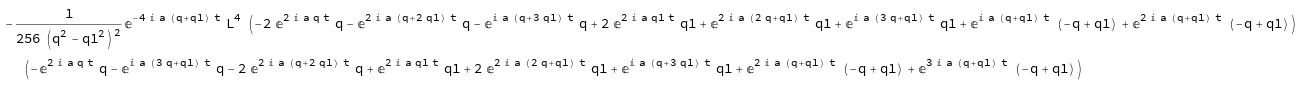
\includegraphics[width=1\linewidth]{row12} \newline
Now I get poles at $q = \pm q_1$, but they can't be gotten rid of like I did before, so we'll have to do a proper principal value. 


% TODO here I separate j = j_1 and j != j_1, but the L factors don't work. It also feels sketchy, since I already took the L-> \infty limit.
%\begin{gather*}
%\sum_{j, j_1 \in (\mathbb{Z}_{even} - \mathbb{N})}
%\big[ \sum_{m \in \mathbb{Z}_{odd}} \frac{L}{4} \frac{qq_1\cos{j\pi/2}\cos{j_1\pi/2}}{(q^2 - k^2)(q_1^2 - k^2)}[e^{-i(\epsilon_k + \epsilon_q)t} + e^{-i(\epsilon_k + \epsilon_{q_1})t} + e^{-2i\epsilon_k t}] 
%+ \delta_{j, j_1}(\frac{L}{4})^3 e^{-2i\epsilon_j t} 
%\big] \big[...^\prime\big] = \\
%\sum_{j \in (\mathbb{Z}_{even} - \mathbb{N})}
%\big[ \sum_{m \in \mathbb{Z}_{odd}} \frac{L}{4} \frac{q^2}{(q^2 - k^2)^2}[2e^{-i(\epsilon_k + \epsilon_q)t} + e^{-2i\epsilon_k t}] 
%+ (\frac{L}{4})^3 e^{-2i\epsilon_j t} \big] \times \\
%\big[ \sum_{m \in \mathbb{Z}_{odd}} \frac{L}{4} \frac{q^2}{(q^2 - k^2)^2}[2e^{i(\epsilon_k + \epsilon_q)t} + e^{2i\epsilon_k t}] 
%+ (\frac{L}{4})^3 e^{2i\epsilon_j t} \big] \\
%+ \sum_{j, j_1 \ne j} \big[ \sum_{m \in \mathbb{Z}_{odd}} \frac{L}{4} \frac{qq_1}{(q^2 - k^2)(q_1^2 - k^2)}[e^{-i(\epsilon_k + \epsilon_q)t} + e^{-i(\epsilon_k + \epsilon_{q_1})t} + e^{-2i\epsilon_k t}] \times \\
%\big[ \sum_{m \in \mathbb{Z}_{odd}} \frac{L}{4} \frac{qq_1}{(q^2 - k^2)(q_1^2 - k^2)}[e^{i(\epsilon_k + \epsilon_q)t} + e^{i(\epsilon_k + \epsilon_{q_1})t} + e^{2i\epsilon_k t}] \big]  = \\
%\sum_{j \in (\mathbb{Z}_{even} - \mathbb{N})}
%\big[ \frac{L}{2\pi}\int_{-\infty}^{\infty} dk \frac{L}{4} \frac{q^2}{(q^2 - k^2)^2}[2e^{-i(\epsilon_k + \epsilon_q)t} + e^{-2i\epsilon_k t}] 
%+ (\frac{L}{4})^3 e^{-2i\epsilon_j t} \big] \times \\
%\big[ \frac{L}{2\pi}\int_{-\infty}^{\infty} dk \frac{L}{4} \frac{q^2}{(q^2 - k^2)^2}[2e^{i(\epsilon_k + \epsilon_q)t} + e^{2i\epsilon_k t}] 
%+ (\frac{L}{4})^3 e^{2i\epsilon_j t} \big] \\
%+ \sum_{j, j_1 \ne j} \big[ \frac{L}{2\pi}\int_{-\infty}^{\infty} dk \frac{L}{4} \frac{qq_1}{(q^2 - k^2)(q_1^2 - k^2)}[e^{-i(\epsilon_k + \epsilon_q)t} + e^{-i(\epsilon_k + \epsilon_{q_1})t} + e^{-2i\epsilon_k t}] \times \\
%\big[ \frac{L}{2\pi}\int_{-\infty}^{\infty} dk \frac{L}{4} \frac{qq_1}{(q^2 - k^2)(q_1^2 - k^2)}[e^{i(\epsilon_k + \epsilon_q)t} + e^{i(\epsilon_k + \epsilon_{q_1})t} + e^{2i\epsilon_k t}] \big] = \\
%\sum_{j \in (\mathbb{Z}_{even} - \mathbb{N})} \big[
%\frac{L^2}{(2\pi)^2}\int_{-\infty}^{\infty} dk \frac{L}{4} \frac{q^2}{(q^2 - k^2)^2}[2e^{-i(\epsilon_k + \epsilon_q)t} +
%e^{-2i\epsilon_k t}] \int_{-\infty}^{\infty} dk \frac{L}{4} \frac{q^2}{(q^2 - k^2)^2}[2e^{i(\epsilon_k + \epsilon_q)t} +
%e^{2i\epsilon_k t}] \\  
%+ \frac{L^3}{4^3}\frac{L}{2\pi}\int_{-\infty}^{\infty} dk \frac{L}{4} \frac{q^2}{(q^2 - k^2)^2}[2e^{i(\epsilon_k  -\epsilon_q)t} + e^{2i\epsilon_k t - 2i\epsilon_q t}] \\
%+ \frac{L^3}{4^3}\frac{L}{2\pi}\int_{-\infty}^{\infty} dk \frac{L}{4} \frac{q^2}{(q^2 - k^2)^2}[2e^{i(-\epsilon_k  +\epsilon_q)t} + e^{-2i\epsilon_k t + 2i\epsilon_q t}] + \\
%\frac{L^6}{4^6} \big] + \\
%+ \sum_{j, j_1 \ne j} \big[ \frac{L}{2\pi}\int_{-\infty}^{\infty} dk \frac{L}{4} \frac{qq_1}{(q^2 - k^2)(q_1^2 - k^2)}[e^{-i(\epsilon_k + \epsilon_q)t} + e^{-i(\epsilon_k + \epsilon_{q_1})t} + e^{-2i\epsilon_k t}] \times \\
%\big[ \frac{L}{2\pi}\int_{-\infty}^{\infty} dk \frac{L}{4} \frac{qq_1}{(q^2 - k^2)(q_1^2 - k^2)}[e^{i(\epsilon_k + \epsilon_q)t} + e^{i(\epsilon_k + \epsilon_{q_1})t} + e^ {2i\epsilon_k t}]
%\end{gather*}
%
%So firstly I notice that we will get a factor of $L^6$ after taking the sums over j to integrals as well, to go with the $L^{-6}$ we got in the beginning, so that's a nice sanity check. I'll drop them from now on. (TODO) the 4th line diverges, but for now I don't let it bother me, since in fact $N_A$ now should diverge after taking the continuum limit, and hopefully it works out.
%
%Now, this is super long to type, so I'll just add print screens from Mathematica here. 
%
%Row 1:\newline
%\includegraphics[width=1\linewidth]{row1}
%Row 2-3:\newline
%\includegraphics[width=1\linewidth]{row23}
%Row 5-6:\newline
%\includegraphics[width=1\linewidth]{row45}
%
%I start with handling rows 4-5: The integration over k is symmetric, thus I can see ()from the expression before the integration) that the expression in symmetric in $q \rightarrow -q$, so I can take the integration over q to $\infty \rightarrow \infty$. We have two poles in $\pm q_1$, but again by definition I can take the specific value. Takes some algebra:
\end{document}